\begin{figure}[H]
\centering
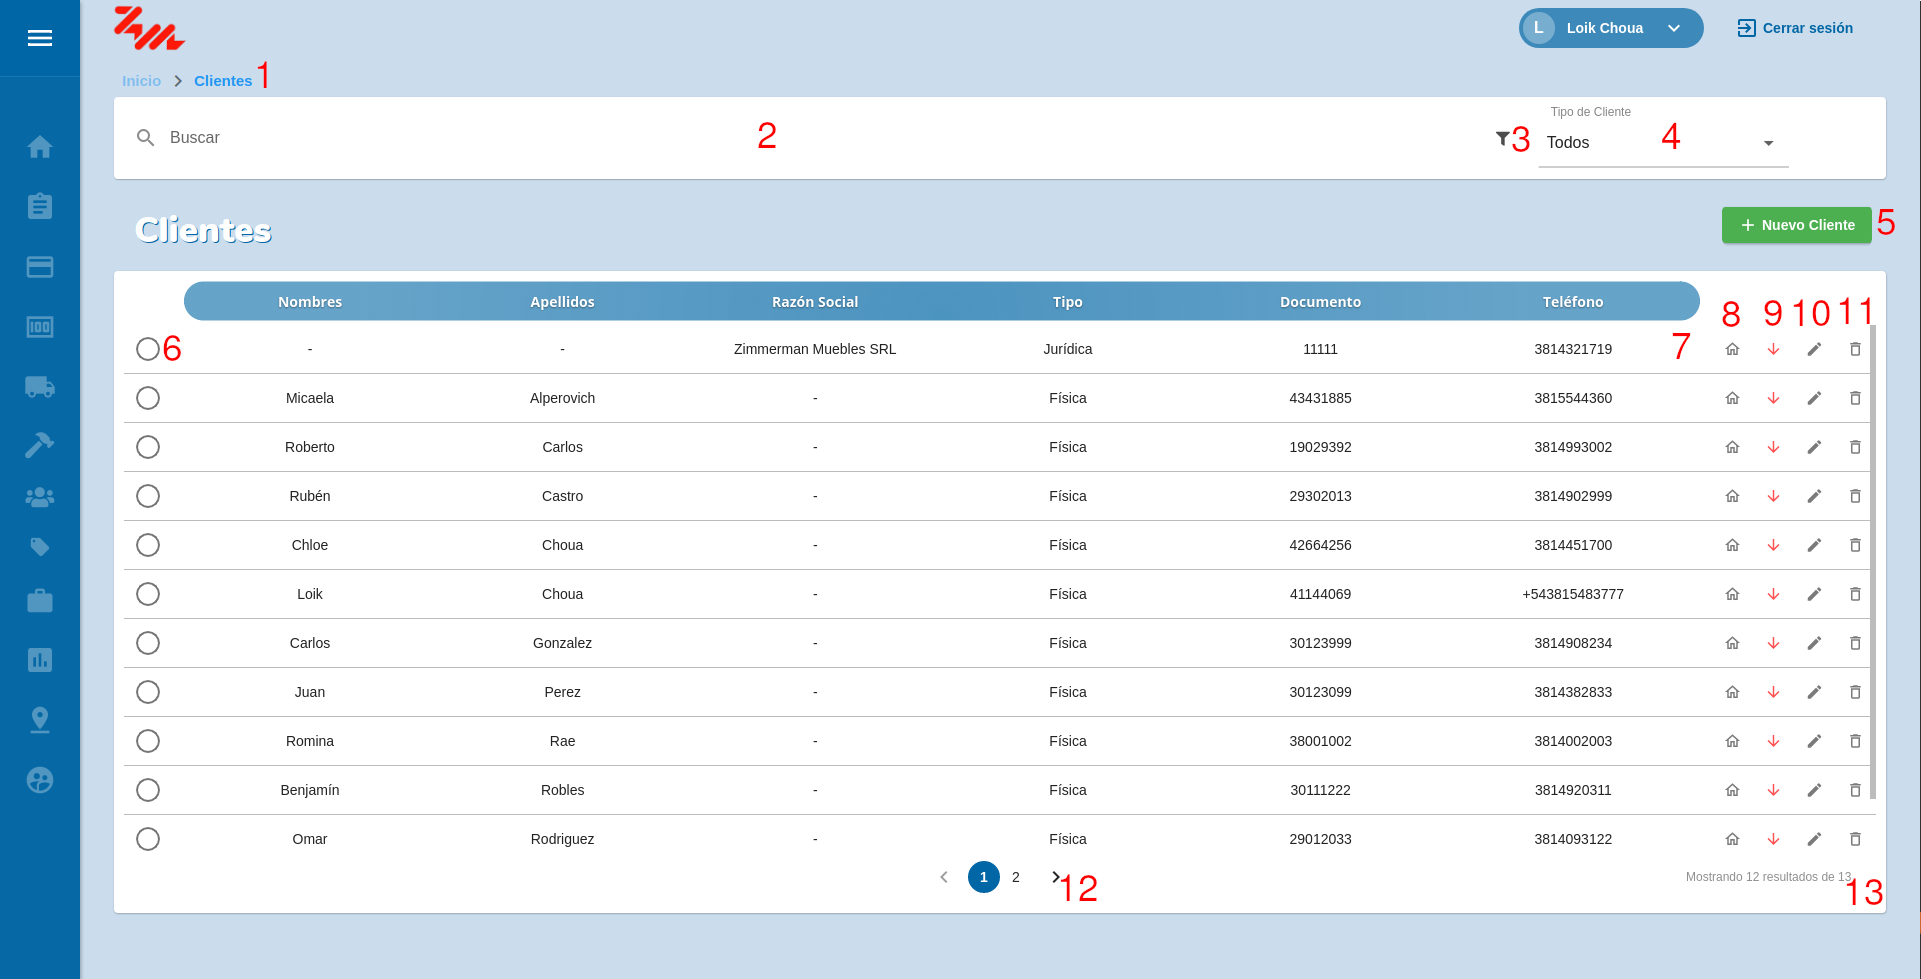
\includegraphics[width=\textwidth,height=\textheight,keepaspectratio]{Escenarios/AD-28-00}
\caption{Escenario - AD-28-00}
\label{fig:AD-28-00}
\end{figure}
Este escenario muestra toda la información referida a los clientes, junto con las acciones disponibles.
El botón \textbf{AD-28-01} permite navegar al escenario \textbf{AD-02-00}. El campo \textbf{AD-28-02} permite ingresar el nombre, apellido o razón social para filtrar los clientes. La lista desplegable \textbf{AD-28-04} permite al usuario filtrar por el tipo de cliente. El botón \textbf{AD-28-03} permite visualizar más filtros de búsqueda disponibles.
El botón \textbf{AD-28-05} permite al usuario crear un nuevo cliente y navega al escenario \textbf{AD-29-00}.
El botón \textbf{AD-28-06} permite al usuario seleccionar uno o más clientes del resultado de la búsqueda. El campo \textbf{AD-28-07} muestra la información relacionada a los clientes  especificando los nombres, apellidos, razón social, tipo de cliente, número de documento y número de teléfono. El botón \textbf{AD-28-08} permite navegar al escenario \textbf{AD-30-00} para ver los domicilios del cliente, el botón \textbf{AD-28-09} permite al usuario dar de alta o de baja el cliente, según el estado en el cual se encuentra. Un click en el botón \textbf{AD-28-10} navega al escenario \textbf{AD-29-00} para editar los datos del cliente y el botón \textbf{AD-28-11} permite al usuario borrar al cliente.
En  \textbf{AD-28-12} se mostrarán las páginas de resultado, pudiendo cambiar de página. En \textbf{AD-28-13} se mostrará cuantos resultados se están visualizando y el total.
\\
